\documentclass{report}
\usepackage[utf8]{inputenc}
\usepackage[T1]{fontenc}
\usepackage[margin=2cm]{geometry}
\usepackage{tcolorbox}
\usepackage{listings}
\usepackage{xcolor}
\usepackage{graphicx}
\usepackage{subcaption}
\usepackage{array}
\usepackage{longtable}

\definecolor{codegreen}{rgb}{0,0.6,0}
\definecolor{codegray}{rgb}{0.5,0.5,0.5}
\definecolor{codepurple}{rgb}{0.58,0,0.82}
\definecolor{backcolour}{rgb}{0.95,0.95,0.92}
 
\lstdefinestyle{mystyle}{
    backgroundcolor=\color{backcolour},   
    commentstyle=\color{codegreen},
    keywordstyle=\color{magenta},
    numberstyle=\tiny\color{codegray},
    stringstyle=\color{codepurple},
    basicstyle=\ttfamily\footnotesize,
    breakatwhitespace=false,         
    breaklines=true,                 
    captionpos=b,                    
    keepspaces=true,                 
    numbers=left,                    
    numbersep=5pt,                  
    showspaces=false,                
    showstringspaces=false,
    showtabs=false,                  
    tabsize=2
}
 
\lstset{style=mystyle}

\newtcolorbox{redbox}[1]{colback=red!5!white,colframe=red!75!black,fonttitle=\bfseries,title=#1}
\newtcolorbox{greenbox}[1]{colback=green!5!white,colframe=green!75!black,fonttitle=\bfseries,title=#1}
\newtcolorbox{bluebox}[1]{colback=blue!5!white,colframe=blue!75!black,fonttitle=\bfseries,title=#1}
\newtcolorbox{graybox}[1]{colback=black!5!white,colframe=black!75!black,fonttitle=\bfseries,title=#1}
\graphicspath{ {/} }

\title{ DIY Laserprojector - ASTEROIDS \\
       \large CAOS Project}
\author{Altava, The\_Reto, L3ivel}
\date{HS 2019}

\begin{document}
\maketitle

\chapter*{Introduction}
\addcontentsline{toc}{chapter}{Introduction}
\section*{Summary}
We are a team of three Computational Sciences students at the University of Basel.
For this project we built a laserprojector using a module of 15 Kpps galvometric mirrors, a RGB-Lasermodule and an Arduino MEGA.
We used this setup to emulate the classic arcade game ASTEROIDS, since the original release of this game made use of vectorized displays any pixel-based emulation is inherently inaccurate.
Using our projector we were able to emulate ASTEROIDS using and directly displaying vector graphics.\\
The first part of this document serves as a project report which has to be turned in for grading.
The second part will go into further detail for anyone interested in how exactly we handled the technical aspects of the project.
The project code as well as this document are available on GitHub (https://github.com/The-Reto/DIY-Laserprojector\_ASTEROIDS).
\section*{Context}
This project was carried out within the scope of the accompanying lecture "Computer Architecture and Operating Systems" (CAOS) held by Professor Florina M. Ciorba and Professor Christian Tschudin at the University of Basel in the autumn semester of 2019.
\section*{Team Members}
The team for this project consisted of:
\begin{itemize}
	\item Altava
	\item The\_Reto
	\item L3ivel
\end{itemize}

\tableofcontents
\newpage

\part{Project Report}
\chapter{Idea \& Inspiration}
\section{What Is a Laserprojector?}
A laserprojector is a device that uses laser beams and a set of mirrors to deflect those beams in order to draw lines over the projecting surface. It is used in industry for high precision tasks such as CNC machines, boat construction or leather nesting. It is also sometimes used for home entertainment as an alternative to beamers.
\subsection{Principle}
A laserprojector uses a single laser source or a combination of red, green and blue (RGB) aligned lasers. The single laser beam is then deflected using two small mirrors attached to galvometric motors. It works a lot like a traditional beamer with the main difference being that it only uses a single source of light.
\subsection{Advantages}
Laser projectors have a few advantages that make them a considerable alternative to traditional beamers. They are extremely accurate and have a wide optical angle, meaning that they can be placed very close to the projecting surface. Furthermore they consume less energy an are overall cheaper than traditional beamers.
\section{Inspiration - Why Build One Yourself?}
The idea to build a laserprojector came from a Youtube video from the creator "StandUpMaths". In his video titled "Recreating Asteroids with Lasers"\footnote{https://youtu.be/FkHjG759ABY} he describes the use of a laserprojector to emulate the classic arcade game ASTEROIDS. The original release of ASTEROIDS used a vector based display for all of its elements and can thus not be emulated to 100\% accuracy on pixel-based monitors. The video also describes the principle of laserprojectors. \\
We also found several similar projects online\footnote{https://www.instructables.com/id/Arduino-Laser-Show-with-Full-XY-Control}\textsuperscript{,}\footnote{https://www.instructables.com/id/Arduino-Laser-Show-With-Real-Galvos}, we used these as further inspiration and reference. Generally speaking we did not use their code directly, the only two exceptions are detailed in the Technical Documentation (see \ref{DAC} and \ref{sound}). \\
Our team decided that the challenge of building a laserprojector would be a good fit for the lecture.
The problem we aimed to solve is evident, we wanted to accurately emulate ASTEROIDS and our main question is "can we do so within our budget and using a laser and a galvometric mirror?".


\chapter{Project Management}
In this chapter we will outline our planning for the project as well as the actual execution and details where and why we deviated from our original plan.
\section{Goals}
We divided our goals into three categories with varying priority. The first category is "Must Have" and is used for the goals we regard as the absolute minimum for our project to be considered a success. The second category, "Nice to Have", are goals ond features we'd very much like to accomplish but are not necessarily crucial for a bare bones version of the project. We labelled the last category as "Perfect Outcome", these are goals and featuers that are in no way necessary and may entail a massive amount of extra work - one could say these are the utopic goals.

\begin{center}
	\begin{longtable}{l l}
		Level & Goals \\
		\hline
		Must Have & Drawing Lissajous-Figures \\
		& Drawing arbitrary closed figures \\
		& Drawing arbitrary figures \\
		\hline
		Nice to Have & RGB-Laser for a visually more appealing results \\
		& Implementation of the ASTEROIDS game core \\
		& Dimming the lasers using PWM for larger color-depth \\
		\hline
		Perfect Outcome & Speaker for generating sounds \\
		& Fully functioning ASTEROIDS emulation \\
	\end{longtable}
\end{center}

\section{Budget}
Before starting the project we decided on a budget of CHF 300. We were in agreement that we'd pay all the hardware ourselves and not take advantage of the university's offering to carry parts of the costs as this would lead to the university owning parts of our hardware resulting in us having to disassemble the project once it would have been graded. By carrying all the costs ourselves we can avoid that. \\
After some discussing we decided that each of us would be willing to invest CHF 100, resulting in a total budget of CHF 300.
\section{Distribution of tasks}\label{distribution}
Because we were confident that we'd reach all of our "Must Have" goals we were able to split the project into three parts and thus assign each team member one part. The three parts we identified were:
\begin{itemize}
	\item Hardware \\
		All things related to hardware issues. What parts to use? How to mount them? Can the whole system be portable? \\
		Altava took responsibility for this part.
	\item IO-Software \\
		Providing software abstractions for the laserpoint on the wall as well as the buttons and other parts. For use in various applications. \\
		The\_Reto took responsibility for this part.
	\item ASTEROIDS-Clone \\
		The main application of our project. A functioning ASTEROIDS clone running on our hardware and using the abstractions provided by the basic IO-Software. \\
		L3ivel took responsibility for this part.
\end{itemize}
Of course there are some overlapping areas between these three parts but they seemed distinct enough to warrant the division. While intensive communication was obviously still necessary, this nonetheless allowed each one of us to have his own schedule and workflow. It also facilitates figuring out each team member's contribution to the project.
\section{Schedule}
We did not plan out our schedule into too much detail in advance. Instead we decided to follow our goals according to their priority and seeing how far we'd get.
\subsection{Hardware}
As soon as the project idea was pitched to the teaching assistants and they gave the go-ahead, the vital hardware parts (mirrors, laser diodes, Arduino, etc.) were ordered. \\
The plan was to assemble the hardware once it has arrived and then start thinking about additional parts by the time the software caught up. For example we first ordered cheap red laser diodes and planned to upgrade as soon as we were confident that the system would work.
\subsection{Software}
Since the software development was split in two parts (see \ref{distribution}), two separate plans were required. One for the IO-Software and one for the ASTEROIDS-clone.
\subsubsection{IO-Software}
The plan for the IO-Software was to start at the lowest level close to the hardware (outputting analog signals to the mirrors) and then add levels of abstractions as time goes on (letting the user set the position of the laserpoint instead of analog levels on the DAC, etc).
\subsubsection{ASTEROIDS}
The idea was to develop a platform independent ASTEROIDS-clone that could then, once the hardware and the IO-Software was done, be displayed using our projects hardware and codebase.
\subsection{Documentation}
The plan for the documentation was to wait until at least the "Must Have" goals were reached and then start to write the documentation and project report as a team effort.
\section{Timeline}
The following list shows a selection of major milestones in the project. Some of the dates are approximate. \\
\\
\begin{center}
	\begin{longtable}{c m{10cm}}
		Date & Milestone \\
		\hline
		\endhead
        07.11.2019 & Project presentation in lecture. \\
        08.11.2019 & First time the whole system is assembled and run. \\
		& Circles and Lissajous-figures are drawn.  \\
        09.11.2019 & Hardware is assembled into the box. \\
        11.11.2019 & Buttons arrive and are mounted onto the box. \\
        14.11.2019 & First successful drawing of a non-Lissajous-figure. \\
		& We are able to draw the house figure that is still in the code. \\
        16.11.2019 & Wiring for the buttons is done and the fan is mounted. \\
        23.11.2019 & The box is painted, and the 3D-printed fan covers are mounted. \\
        29.11.2019 & RGB-laser module arrives. First test of the colored laser. \\
		& It is not yet mounted into the box. \\
        30.11.2019 & TextRenderer is working. First display of text. \\
        10.12.2019 & Sound module is working. We're annoying everyone in our vicinity with the piezo buzzer. \\
        19.12.2019 & The RGB-Laser module is mounted into the box. \\
		11.01.2020 & The Asteroids clone is run for the first time. \\
	\end{longtable}
\end{center}

\begin{figure}[h]
	\centering
	\begin{subfigure}[b]{0.45\textwidth}
		\centering
		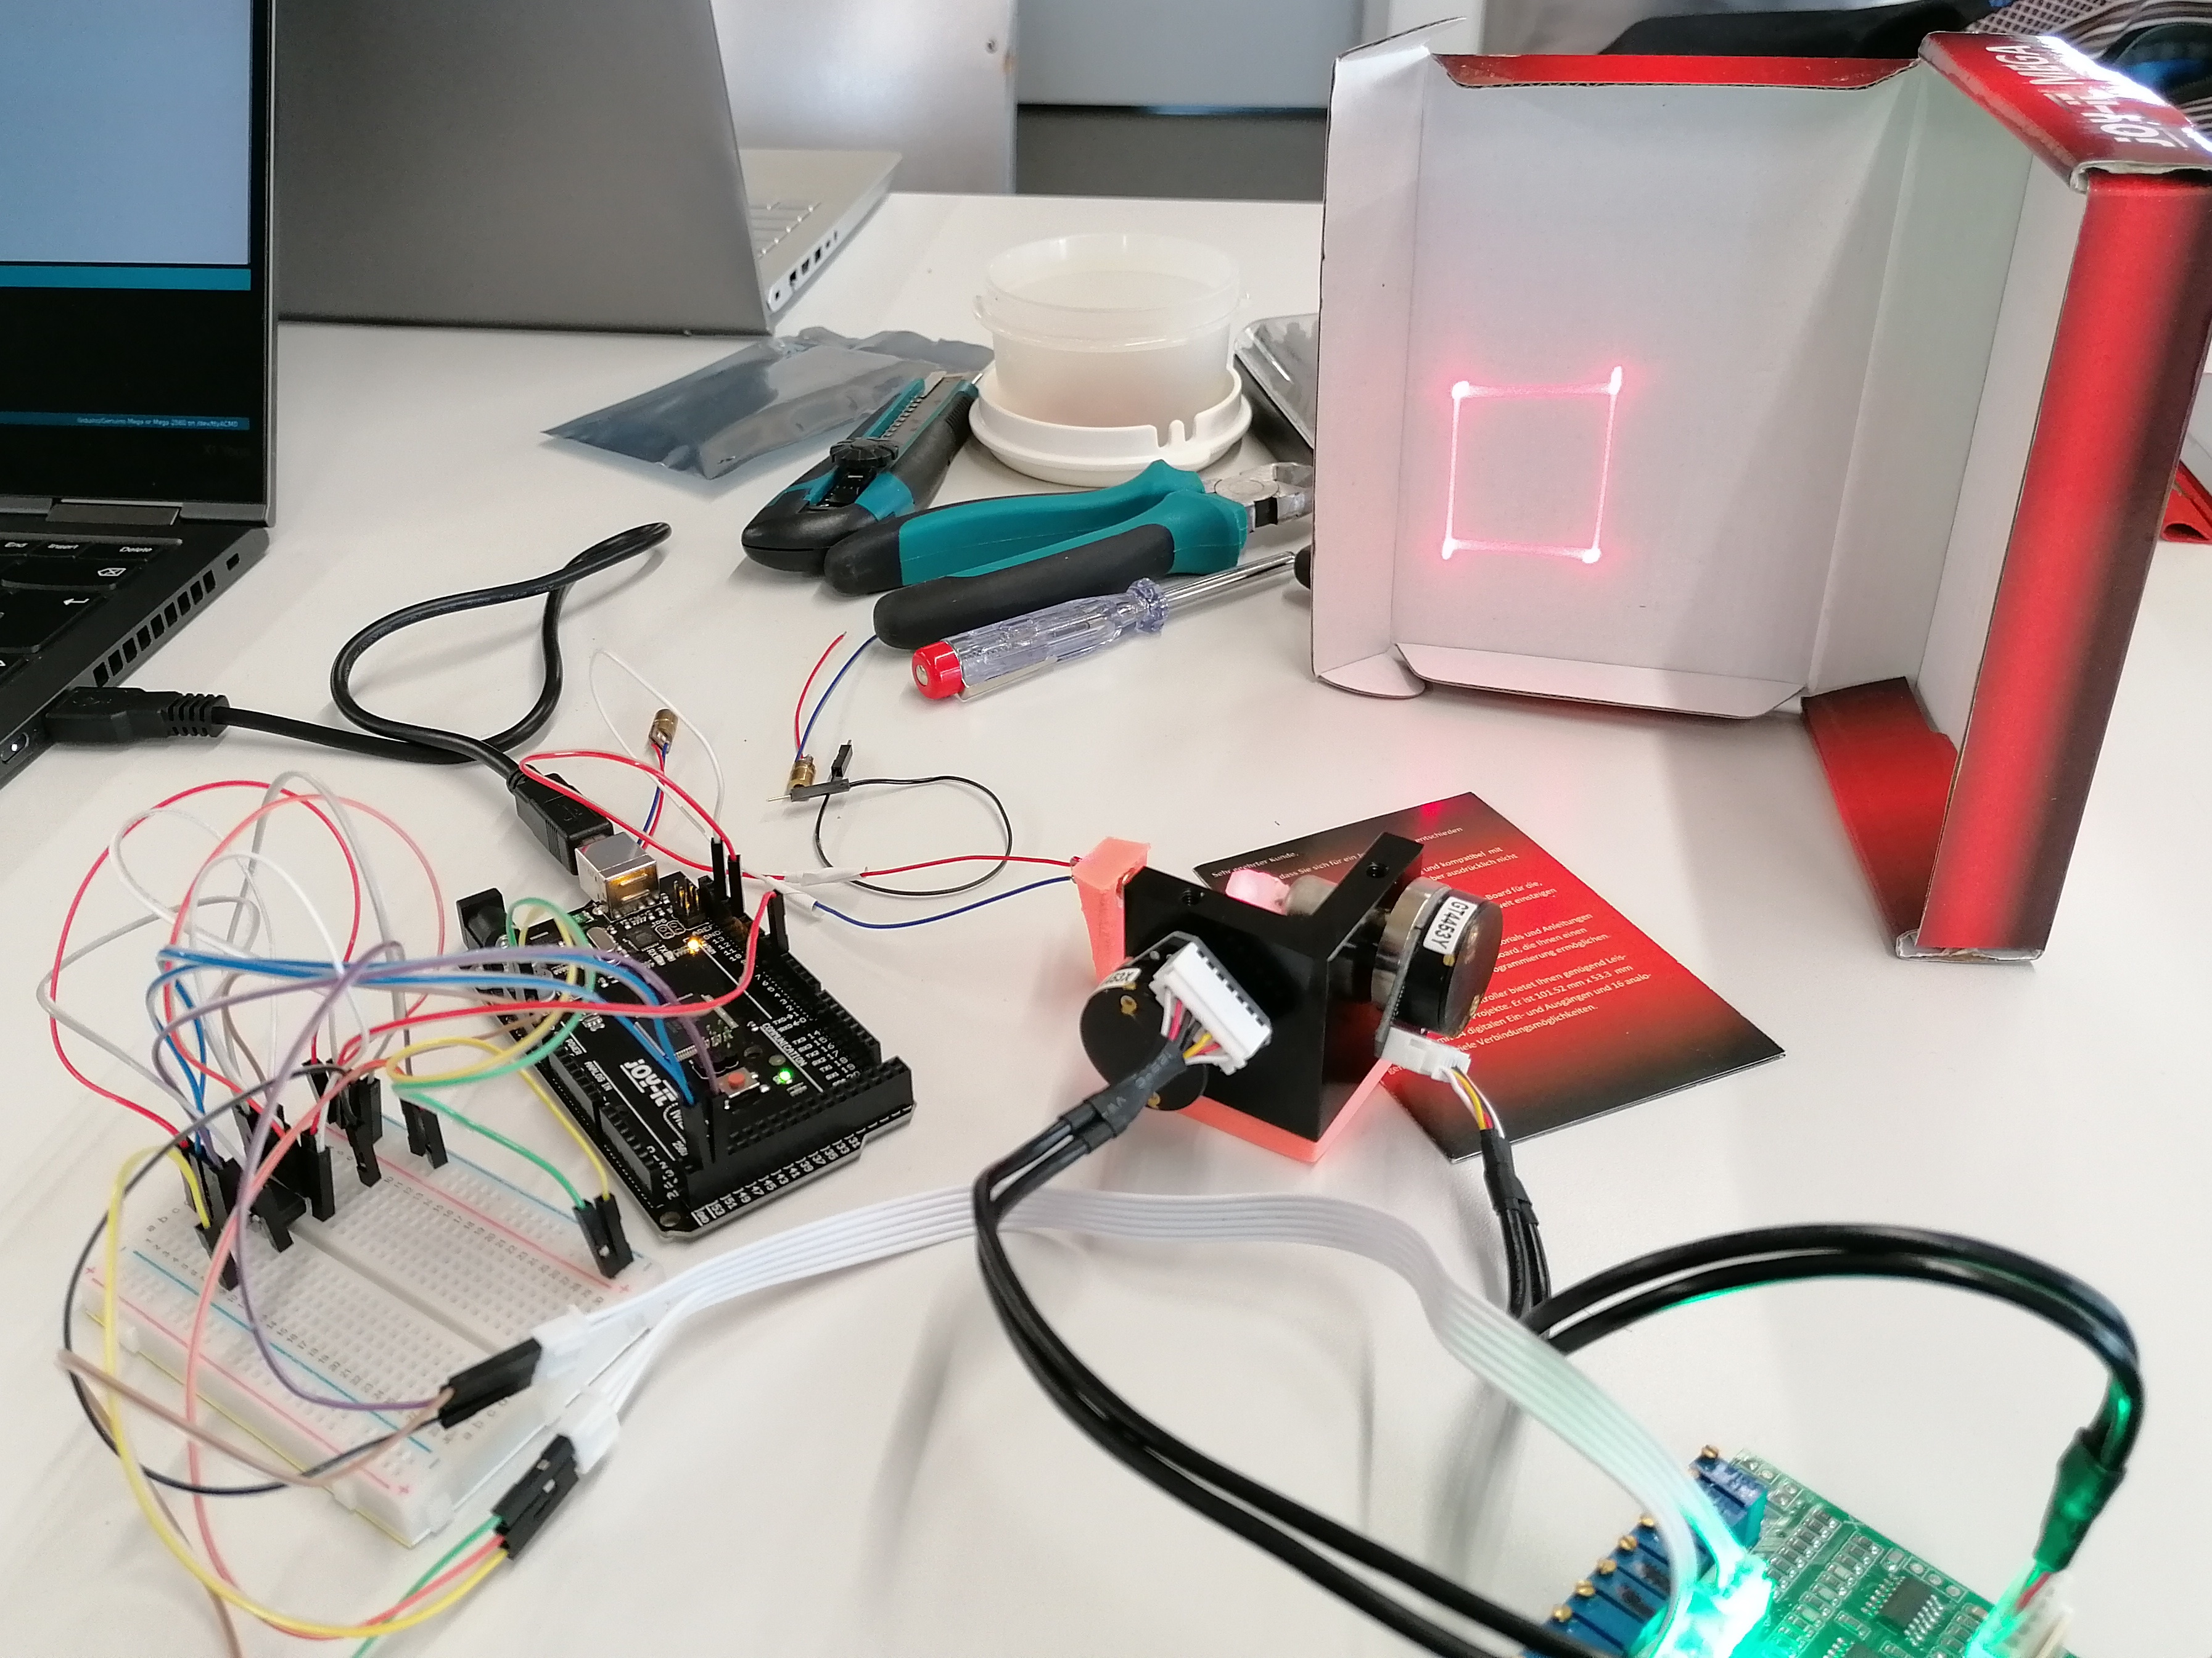
\includegraphics[width=0.9\textwidth]{assembly.jpg}
		\caption{First assembly of the core parts. Note the imperfections at the edges of the square}
		\label{img:assembly}
	\end{subfigure}
	~
	\begin{subfigure}[b]{0.45\textwidth}
		\centering
		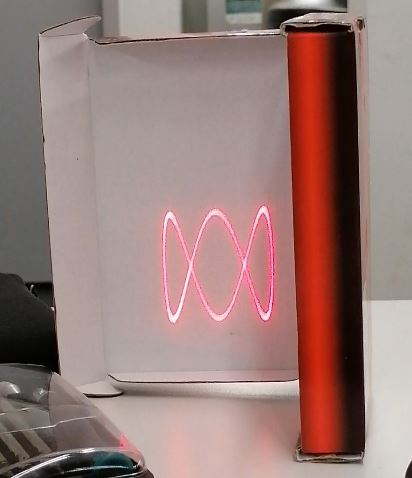
\includegraphics[width=0.6\textwidth]{lissajous.jpg}
		\caption{Drawing Lissajous figures.}
		\label{img:lissajous}
	\end{subfigure}

	\begin{subfigure}[b]{0.45\textwidth}
		\centering
		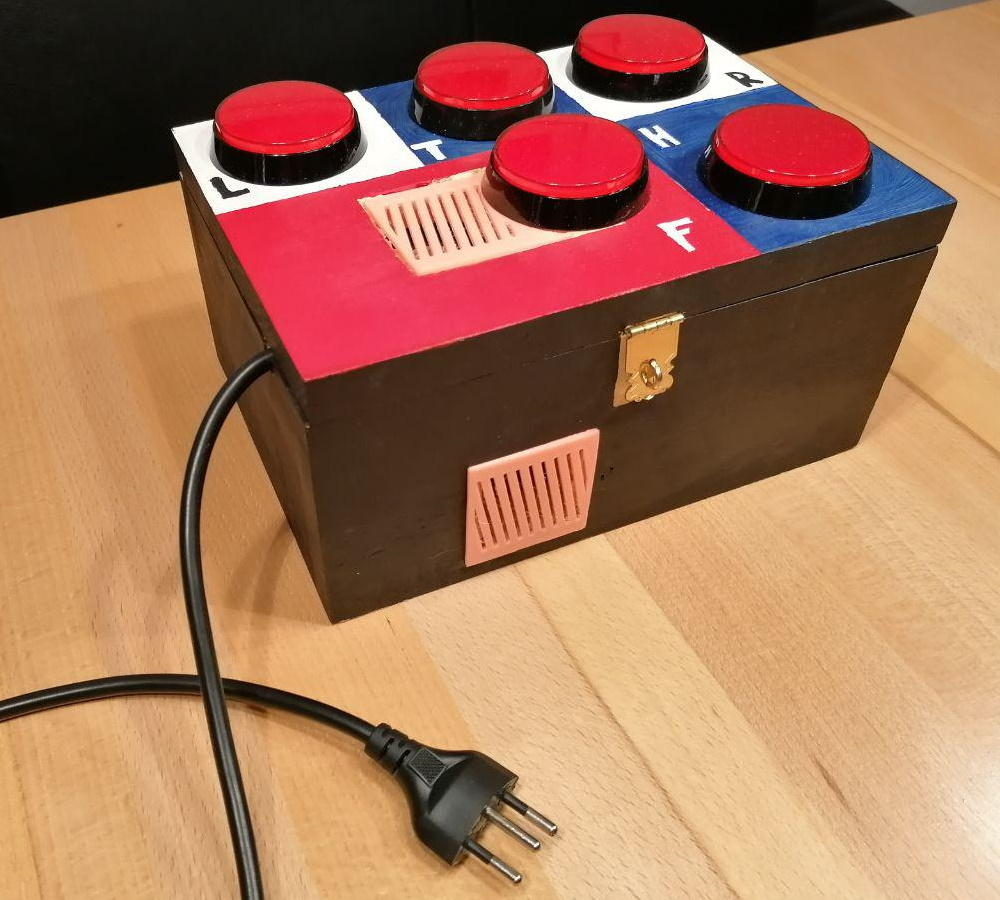
\includegraphics[width=0.8\textwidth]{box.jpg}
		\caption{The finished laser projector.}
		\label{img:box}
	\end{subfigure}
	~
	\begin{subfigure}[b]{0.45\textwidth}
		\centering
		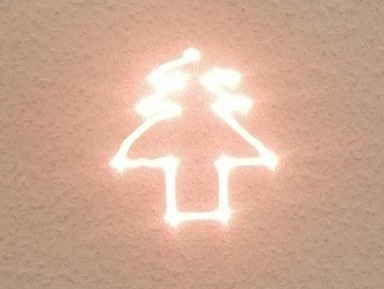
\includegraphics[width=0.8\textwidth]{tree.jpg}
		\caption{The Christmas tree figure.}
		\label{img:tree}
	\end{subfigure}
\end{figure}
\chapter{Result \& Outlook}
Our main goal was to create a fully functioning ASTEROIDS clone. We did not completely reach this goal. While playable, our clone is far from being complete. All in all we are still happy with our result. Details on the hardware and the software can be found in part \ref{documentation} of this document. \\
However, there is a lot more we can do with the hardware and libraries we created. With our sound library and the saved RTTTL songs, we could set up a jukebox with a menu where you can select melodies to play (see \ref{sound}). \\
Another option is to finish the SVG-converter (see \ref{svg-conv}). This would allow for the user input of any .svg file that could then be displayed by our projector. \\
Finally we could combine all of these features in a selection menu and turn our box into a multimedia station.
\section{Challenges \& Deviations From Original Idea}
Drawing Lissajous figures worked quite early, so we were confident that drawing closed figures would be easily achievable. Our first idea was to use a two dimensional Fourier transform to display arbitrary closed figures, but it turned out that our fixedpoint arithmetics library lacked the neccessary precision to deliver satisfactory results. \\
We thus decided that we'd forego the Fourier transform and instead just move the laser point from vertex to vertex in a straight line. Yet it turned out to be a major obstacle to even draw clean straight lines. It appeares that the mirrors "overshoot" the target position, so when we tell them to move from position (x\textsubscript{0},y\textsubscript{0}) to position (x\textsubscript{0},y\textsubscript{1}), the laserpoint would stop at (x\textsubscript{0},y\textsubscript{1}+a) and then move back, leveling out at the desired position. We suspect that this effect is due to the angular momentum of the mirrors. Our current solution is to add points inbetween, so that the mirrors don't accelerate too much and therefore reduce overshooting. \\
Another challenge was the arrangement of the parts in the box. We started assembling the parts into the box pretty early and a lot of the setup changed afterwards. When we installed the cooling system, which is very space consuming, we had to cut out vents and find a suiting place for the fan. All of this had to be done without knowing the dimensions of the RGB laser module, as it arrived very late and had no technical specifications provided by the seller. The interior of the box underwent several iterations, but ended up in a pretty good state, despite all the unknown variables. \\
After testing we found that our idea of using PWM to allow dimming of the lasers turned out to be impossible. While applying a modulated output to a stationary laser point creates the illusion of dimming the point, this technique stops working as soon as the laser point is in motion. It turns out the dimming effect on the laser point arrises from the point being turned on and off in rapid succession. When we move the laser point around using the mirrors this results in dashed or dotted lines - while this is a cool effect, it is not what we were aiming for. \\
The idea of adding sound came very late, but ended up being a good decision as it didn't really intervene with the rest of the project and adds very nice to the arcade feeling of our ASTEROIDS clone. \\
The installation of an RGB laser was decided on in the early stages of the project. We agreed that it would enhance the quality without adding much complexity. It turned out to do just that.


\part{Appendix: Technical Documentation}\label{documentation}

\chapter{Hardware}\label{hardware}
\section{Parts Overview}



\begin{figure}[h]
	\centering
	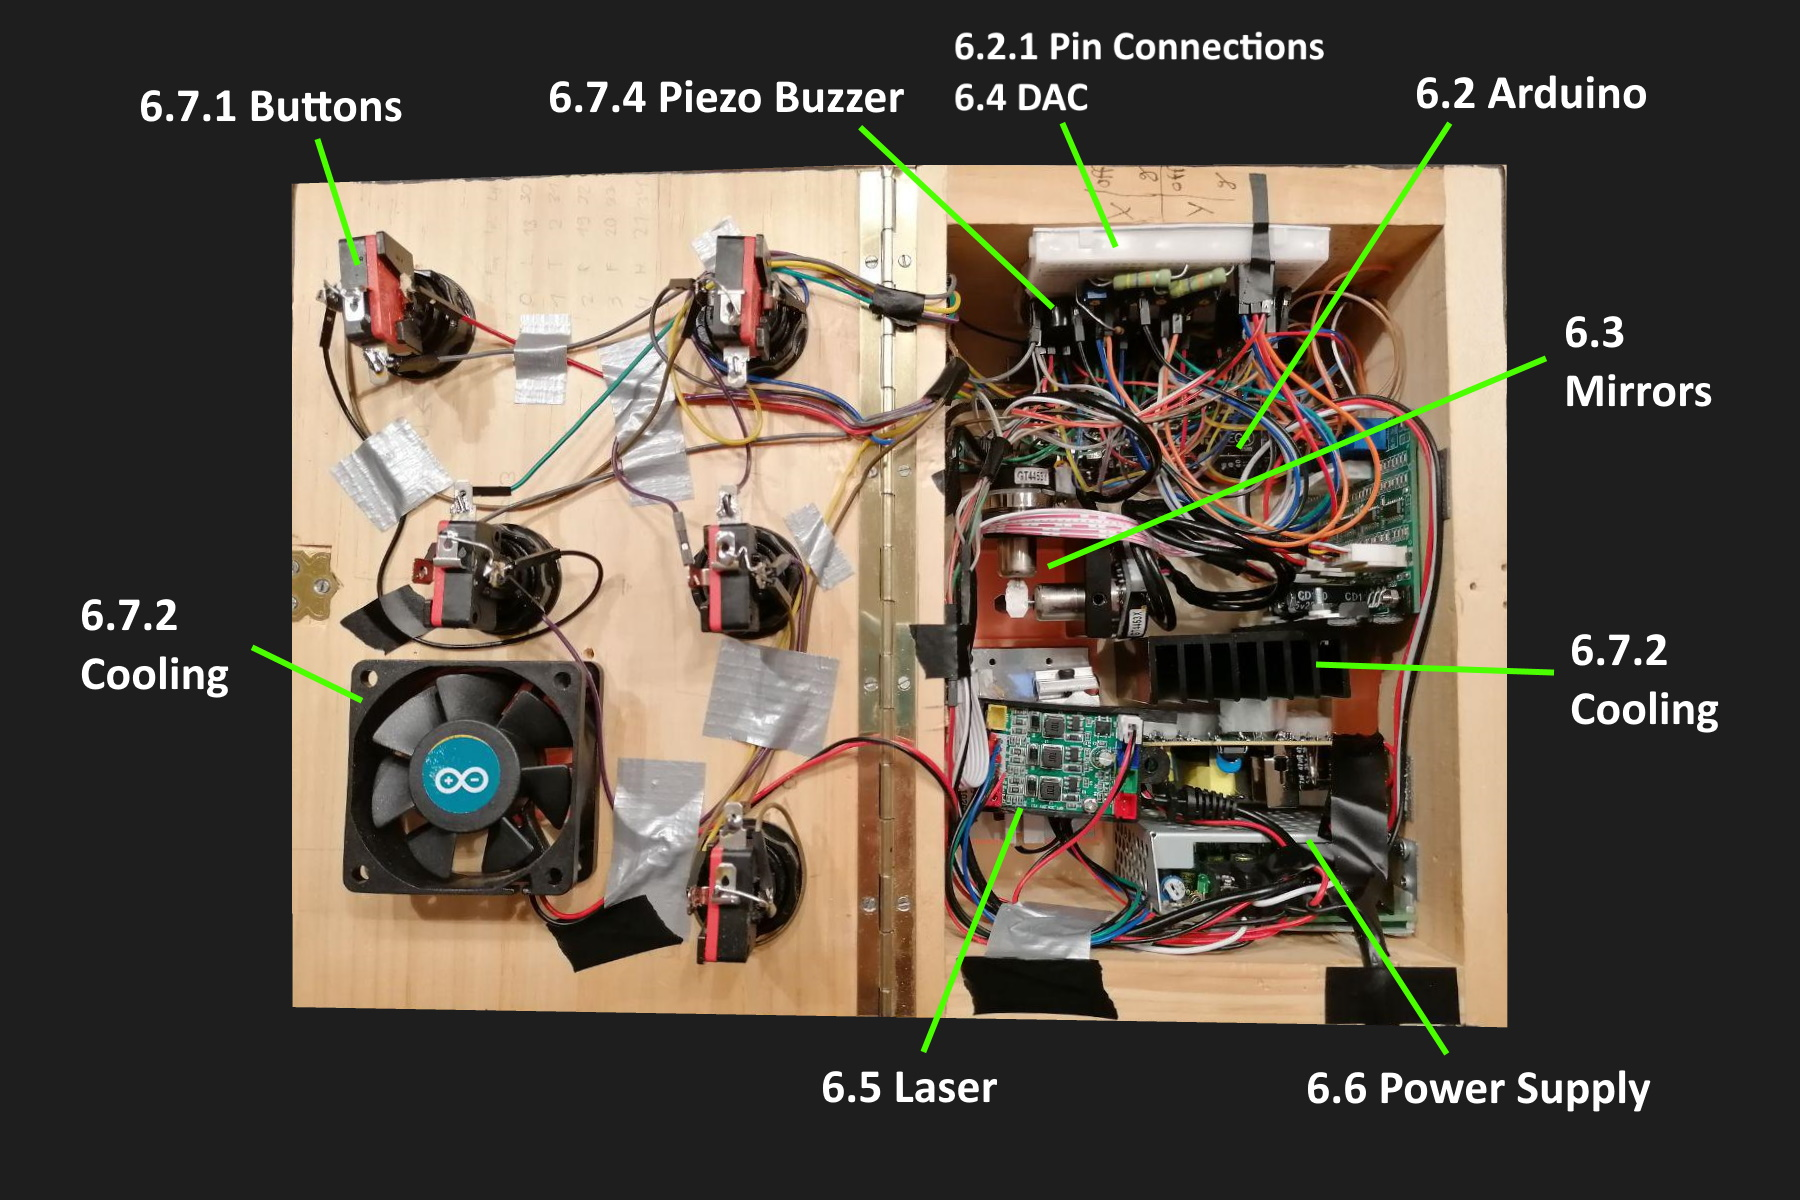
\includegraphics[width=\textwidth]{parts.jpg}
	\caption{The interior of our laser projector. On the left side is the lid where the buttons and the fan are embedded. On the right side are all the other parts mounted in the box.}
	\label{img:parts}
\end{figure}

All the parts of our laser projector are mounted in a 24cm x 17cm x 12cm wooden box. The buttons are embedded in the lid as well as the heat exhaust. On the back side is a sealable opening where the laser beam will come out of. The whole projector is powered by a single standard Swiss type power plug.

\section{Arduino}

The Arduino MEGA2560 controlling our projector is mounted on the bottom of the box and barely visible under the wires. It is connected to the DAC, the laser, the piezo buzzer and the buttons as well as their lights.

\subsection{Pin Connections}

Most of the Arduino output is connected to a standard breadboard using jumper wires. The DAC and the piezo buzzer are located on the breadboard, as well as some amplifier circuits. \\
The pins of the Arduino are connected as follows.

\begin{center}
	\begin{longtable}{l r}
		Part & Pin Number \\
		\hline
		Piezo Buzzer & 47 \\
		SDI (DAC) & 51 \\
		SCK (DAC) & 52 \\
		CSP (DAC) & 53 \\
		LDAC (DAC) & 5 \\
		Red Laser & 40 \\
		Green Laser & 41 \\
		Blue Laser & 42 \\
		Button Interrupts & 2, 18-21 \\
		Button Lights & 30-34 \\
	\end{longtable}
\end{center}

\section{Mirrors \& Galvometric Motors}\label{mirrors}

Two small mirrors mounted on galvometric motors are the heart of our projector. The mirrors are capable of 25kppm (kilo points per second), meaning they can draw 25'000 distinguishable points per second on the projection surface. The motors are controlled by an accompanying PCB (printed circuit board). It can be seen right of the mirrors, mounted on the wall. The PCB has two MOSFETs (Metal–Oxide–Semiconductor Field-Effect Transistor) and a small heatsink attached. Those MOSFETs develop a reasonable amount of heat in just a few minutes of operation, surpassing the capabilities of the already installed heatsink. This lead us to attaching a much bigger heatsink to the existing one and the additional installment of a fan.

\section{DAC}\label{DAC}

The DAC (Digital-to-Analog Converter) is needed as a translator between the Arduino and the galvometric motors. It converts the digital signals of the Arduino to analog signals needed by the galvometric motors. We use a MCP4922 DAC.

\section{Laser}

\begin{figure}[h]
	\centering
	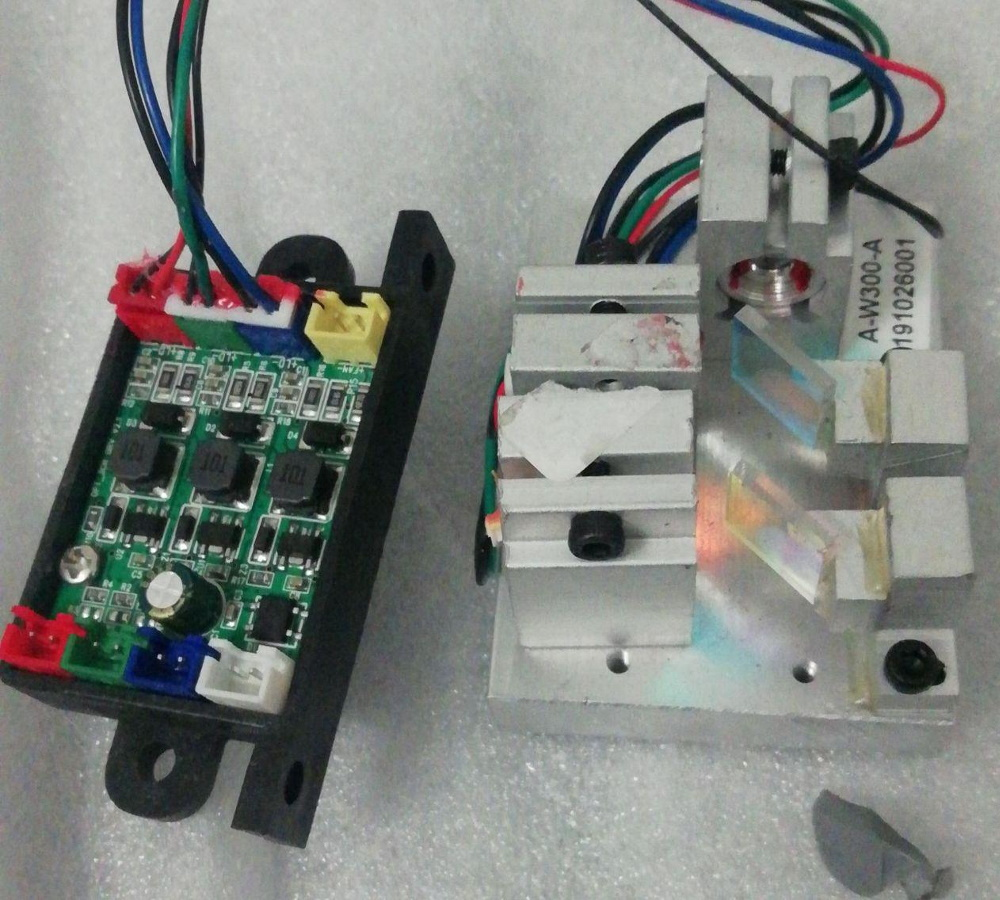
\includegraphics[width=0.5\textwidth]{laser.jpg}
	\caption{The laser and its controller.}
	\label{img:laser}
\end{figure}

We use an RGB laser so we can project different colors instead of only one. In the early stages of our project we used a cheap red laser and were not satisfied with the results, so we decided to upgrade our projector. The accompanying PCB is connected to the Arduino and lets us turn the differently colored lasers (red, green and blue) on and off separately.

\section{Power Supply}

The power cord is connected to two different power supply units. One has a 15V output and powers the galvometric motors and the fan. The other one has a 5V output and powers the laser as well as the Arduino.

\section{Additional Parts}

\subsection{Buttons}

\begin{figure}[h]
	\centering
	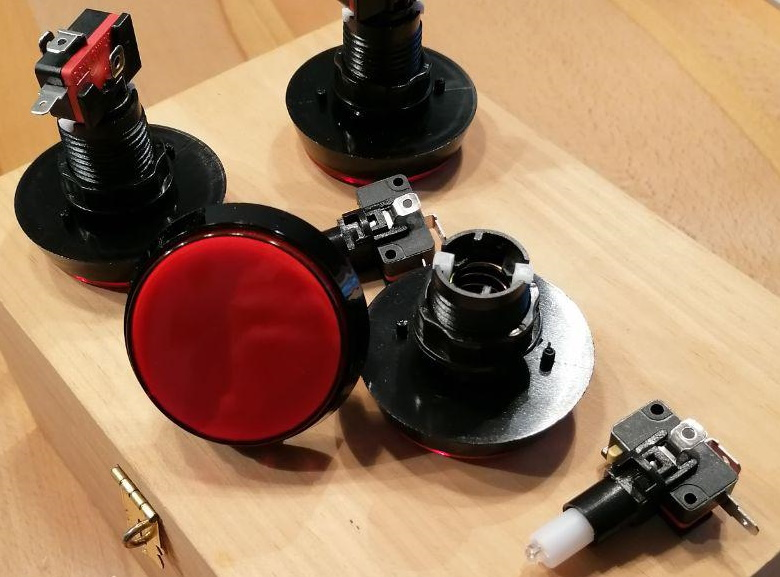
\includegraphics[width=0.5\textwidth]{buttons.jpg}
	\caption{Some disassembled buttons.}
	\label{img:buttons}
\end{figure}

For playing Asteroids you need five buttons. We used the 60mm Red Arcade Buttons by Adafruit for a real arcade-like feeling.\footnote{This project is not sponsored or supported by Adafruit in any way.} The buttons are equipped with an LED and can be lit individually by the Arduino.

\subsection{Cooling}

As mentioned in section \ref{mirrors}, the operation of the galvometric mirrors produces a significant amount of heat. In order to cool the MOSFETs, we attached a large heat sink to the existing one. This alone is a vast improvement and allows for operation over several hours with reasonable temperature development. Still we decided to install a fan and two vents to dissipate the hot air in order to protect the parts and box from taking damage.

\subsection{Box}

The box is handmade out of 2cm thick maplewood. It is painted with acryllic color in the style of the original Asteroids arcade cabinet.

\subsection{Piezo Buzzer}

A late addition to the project was a piezo buzzer for simple arcade sounds, further improving the emulation of an Asteroids arcade cabinet. It is controlled by the Arduino and can generate simple notes by turning the input signal on and off at certain frequencies.

\subsection{Other Parts}

Several parts are 3D-printed. This includes the laser protection cover, the louvres and the stand aligning laser and mirrors.

\section{Cost Overview}

The total cost for the project ended up as follows.

\begin{center}
	\begin{longtable}{l r}
		Part & Price (all prices in CHF) \\
		\hline
		laser diode red & 6.00 \\
		galvometric motors with mirrors & 125.90 \\
		RGB laser module & 48.90 \\
		power supply for laser & 28.90 \\
		Arduino MEGA & 20.00 \\
		DAC & 16.00 \\
		Arcade Buttons & 29.10 \\
		Heat Sink & 5.55 \\
		Other (Resistors, Wires, Shipping etc.) & 62.40 \\
		\hline
		Total & 342.75 \\
	\end{longtable}
\end{center}

\chapter{Software}
\section{Software Overview \& Structure}
\section{IO Software}
\subsection{Graphics}
We provide an abstraction for the laser and the mirrors. Instead of worrying about the mirrors and the laser directly, the user should only worry about the laserpoint on the wall. The most important function in that regard is probably the following which controls the laserpoint on the wall.
\begin{lstlisting}[language=c++]
moveLaser(Laser *l, Command c)
\end{lstlisting}
A further abstraction is provided with the \verb Drawing  and \verb Scene  structs used to hold even higher level abstraction for pictures to be drawn. In the following paragraphs the details of each level of abstraction are provided.
\subsubsection{DAC}
As outlined in the hardware section (\ref{hardware}) of this documentation, the mirrors are not directly connected to the Arduino. Instead the mirrors are connected to a DAC, the analog output is then used to control the angle of the mirrors. \\
To control the DAC we copied, adapted and build upon public domain code found on GitHub\footnote{https://github.com/helgenodland/MCP4922-Arduino-SPI-Library}.\\
The \verb DAC.cpp  file provides functions controlling the DAC and setting its output level. This file defines a struct \verb DAC  containing the appropriate pin connections. The file provides the function \lstinline[language=c++]{DAC *generateDAC(int _SDI, int _SCK, int _CS, int _LDAC)} that can be used to initialize a \lstinline[language=c++]{DAC}-struct to then be used. The function also initializes the \lstinline[language=c++]{SPI}-library, which is used to transfer the data to the DAC.\\
The function \lstinline[language=c++]{void Set(DAC *dac, unsigned int A, unsigned int B)} is used to set the DAC provided in the argument \lstinline[language=c++]{*dac} to the levels provided in the two arguments \lstinline[language=c++]{A} and \lstinline[language=c++]{B}, using the first output channel of the DAC for the value in \lstinline[language=c++]{A} and the second one for the value on the \lstinline[language=c++]{B} argument. The two arguments must be between 0 and 4095, as we are using a 12-bit DAC. \\
The library defines the following datastructures:
\begin{itemize}
	\item \lstinline[language=c++]!struct MCP4922 {int _SDI, _SCK, _CS, _LDAC}! \\
		holds the pin connections for the MCP4922 DAC we're using.
	\item \lstinline[language=c++]{typedef struct MCP4922 DAC} \\
		provides an easier name for the struct used to hold the pin connections.
\end{itemize}
The library provides the following functions:
\begin{itemize}
	\item \lstinline[language=c++]{DAC* generateDAC(int _SDI, int _SCK, int _CS, int _LDAC)} \\
		returns a pointer to a DAC object using the provided pin numbers.
	\item \lstinline[language=c++]{void Set(DAC* dac, unsigned int A, unsigned int B)} \\
		sets the output channel A of the DAC provided in \lstinline[language=c++]{dac} to the value in the argument \lstinline[language=c++]{A}.\\
		sets the output channel B of the DAC provided in \lstinline[language=c++]{dac} to the value in the argument \lstinline[language=c++]{B}.
\end{itemize}
\subsubsection{Laser}
The files \verb Laser.cpp  and \verb Laser.h  are probably the most important pieces of code in the whole project, as they provide the necessary functions to fully control the laser point on the wall. They provide functions, datastructures and constants for controlling position, movement and color of the laser. \\
The goal is to provide a level of abstraction to allow the user to control the laser point on the wall, instead of having to worry about the angle of the mirrors or the laser module. \\
The library provides the following datastructures:
\begin{itemize}
	\item \lstinline[language=c++]{typedef unsigned char COLOR} \\
		Just a typedef for \lstinline[language=c++]{unsigned char} to indicate its use as a color. \\
		An \lstinline[language=c++]{unsigned char} holds 8 bits, the first two are unused for \lstinline[language=c++]{COLOR}, the remaining 6 bits are shared equally across the three color-channels RGB, with two bits each. The structure is thus: \lstinline[language=c++]{EE RR GG BB} \\
		Example: 51 = \lstinline[language=c++]{00 11 00 11} is equivalent to the color purple (\lstinline[language=c++]!{255, 0, 255}!).\\
		\emph{Note:} On the current hardware we have no possibility of dimming the laser, nor the individual color-channels. This means that, currently, the laser corresponding to one color-channel will be fully activated whenever either one or both of the corresponding bits is set - effectively reducing our color-depth from 6 bits to 3. \\
	\item \lstinline[language=c++]{typedef unsigned long COMMAND} \\
		A typedef masking an \lstinline[language=c++]{unsigned long} as a \lstinline[language=c++]{COMMAND}. These commands are used to encode a new position for the laser to move to  as well as a color during the move - thus allowing to encode any movement of the laser into 32 bits. This has two main advantages; first it is efficient with memory, and secondly it allows the SVG-Converter (see \ref{svg-conv}) to output a CSV file containing numbers, which then in turn can easily be used on the hardware. \\
		The 32 bits of a \lstinline{unsigned long} are used as follows:
		\begin{itemize}
			\item The first 12 bits encode the x-position. 
			\item the next 12 bits encode the y-position. 
			\item the following 6 bits encode the color (see \lstinline{COLOR}) 
			\item the bit at the second to last position is the \lstinline{COLOR_CHANGE}-bit. 
				As changing the color of the laser takes a comparably large time (approx. 200 microseconds) the lasers color is not set for every point - rather it is only changed when the \lstinline{COLOR_CHANGE}-bit is set.
			\item the last bit is the \lstinline{LASER_OFF}-bit, if it is set the laser will always be turned off (color black). 
\end{itemize}
The overall structure of a \lstinline{COMMAND} is thus: (\lstinline{x} for the x-position, \lstinline{y} for the y-position, \lstinline{rgb} for the color and \lstinline{t} for the two technical bits) \\
\lstinline{xxxx xxxx xxxx yyyy yyyy yyyy rrgg bbtt}
	\item \lstinline[language=c++]{struct Laser}\\
		with the following structure: \\
\begin{lstlisting}[language=c++]
struct Laser {
    int x, y;
    COLOR color;
#ifdef USE_SIMULATOR
    int frame;
    IMAGE target;
#else
    DAC dac;
#endif //USE_SIMULATOR
};
\end{lstlisting} 
This structure is used to describe one laser point (yes, we could theoretically use more than one). It holds the current position of the point and its current color. Depending on whether the simulator (see \ref{simulator}) is used or the actual hardware, the struct also holds either a \lstinline[language=c++]{DAC}-object for use with the real hardware, or a frame for the simulator.
\end{itemize}
The library provides the following functions:
\begin{itemize}
	\item \lstinline[language=c++]{LASER* generateLaser()} \\
		returns a laser struct with all the necessary variables initialized. The position is set to be at 2000, 2000 and the color is set to be black (i.e. laser turned off).
	\item \lstinline[language=c++]{void setLaserColor(LASER *l, COLOR col)} \\
		Sets the laser to the color provided.\\
		\emph{Note:} Our current hardware does not support dimmed color, see previous note on the color data structure.
	\item \lstinline[language=c++]{int deleteLaser(LASER* l)} \\
		Deletes the provided laser, freeing all allocated space.
	\item \lstinline[language=c++]{void moveLaser(LASER* l, COMMAND cmd)} \\
		Moves the laser point from its current position to the position encoded in the \lstinline{COMMAND}. During the move the laser will keep its previous color, unless the \lstinline{COLOR_CHANGE}-bit is set. In this case the laser will first change its color to the color encoded in the \lstinline{COMMAND}.
	\item \lstinline[language=c++]{COLOR getColor(COMMAND cmd)} \\
		Returns the color value encoded in the  \lstinline{COMMAND} cmd as a \lstinline{COLOR}.
	\item \lstinline[language=c++]{COMMAND getCommand(unsigned short xPos, unsigned short yPos, COLOR col)} \\
		Returns a valid \lstinline{COMMAND} encoding the position \lstinline{(xPos, yPos)} and the \lstinline{COLOR col}. Neither the \lstinline{COLOR_CHANGE} nor the \lstinline{LASER_OFF}-bit is set. If desired, they have to be set manually by adding the appropriate constant.
	\item \lstinline[language=c++]{COMMAND addCorrection(int x, int y, COMMAND c)} \\
		Adds an offset to the position in the provided \lstinline{COMMAND}.
\end{itemize}
\subsubsection{Drawing}
The library \verb Drawing  provides further abstractions for the graphical output of our projector. Providing a \lstinline[language=c++]{struct} called \lstinline{drawingObject} holding position, rotation, scale etc. of a drawable object. Furthermore it allows for the grouping of several \lstinline{drawingObcect}s into a \lstinline{scene} consisting of an array of \lstinline{drawingObject}s and, crucially, an array of \lstinline{COMMAND}s that can directly be drawn using the laser class.\\
The library provides the following datastructures:
\begin{itemize}
	\item \lstinline[language=c++]{struct drawingObject} \\
		with the following structure:
\begin{lstlisting}[language=c++]
struct drawingObject {
    char type;
    Vector pos;
    short rot;
    short scale;
    int len;
    COLOR color;
    const short* data;
};
\end{lstlisting}
	\item \lstinline[language=c++]{struct scene} \\
		with the following structure:
\begin{lstlisting}[language=c++]
struct scene {
    int noOfObjects;
    int noOfPoints;
    drawingObject objects[16];
    COMMAND* cmds;
};
\end{lstlisting}
\end{itemize}
The library provides the following functions:
\begin{itemize}
	\item \lstinline[language=c++]{scene* makeScene()} \\
		Returns a pointer to an empty scene object.
	\item \lstinline[language=c++]{void deleteScene(scene* s)} \\
		Deletes a scene, freeing all allocated memory. Scenes must be destroyed this way.
	\item \lstinline[language=c++]{void addObjectToScene(scene* scene, drawingObject object)} \\
		Adds a \lstinline{drawingObject} to the scene provided.
	\item \lstinline[language=c++]{void buildScene(scene* s)} \\
		Renders the scene by iterating through all the objects in the scene and generating the array of commands. \\
		\emph{Note:} This function must be called before the \lstinline{scene} is drawn the first time. It must also be called when there have been updates to the position, rotation or any other relevant field of an object.
	\item \lstinline[language=c++]{void drawScene(scene toDraw, LASER l)} \\
		Draws the scene using the laser provided.
\end{itemize}
The library provides the following constants and variables:
\begin{itemize}
	\item \lstinline[language=c++]{static drawingObject HOUSE} \\
		A \lstinline{drawingObject} providing the image of a simplified house.
	\item \lstinline[language=c++]{static drawingObject SHIP} \\
		A \lstinline{drawingObject} providing the image of a spaceship - this is the graphic used in the ASTEROIDS game.
	\item \lstinline[language=c++]{static drawingObject ROCK} \\
		A \lstinline{drawingObject} providing the image of an abstract boulder - this is the graphic used for the eponymous asteroids in the game.
	\item \lstinline[language=c++]{static drawingObject TREE} \\
		A \lstinline{drawingObject} providing the image of a simplified (Christmas) tree. This object was added shortly before Christmas to aid with the festive spirit during development.
\end{itemize}
\begin{figure}[h]
	\centering
	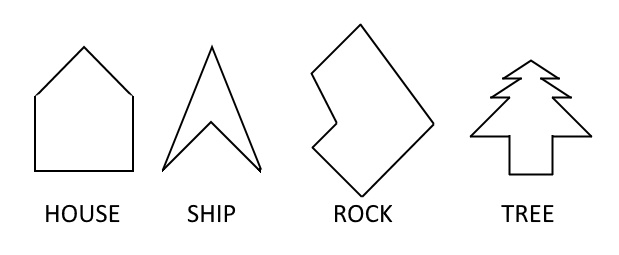
\includegraphics[width=\textwidth]{forms.jpg}
	\caption{Visualization of the forms we can draw.}
	\label{img:forms}
\end{figure}
\subsubsection{TextRenderer}
The TextRenderer library is used to render text onto a \lstinline{scene}.
The library provides the following function:
\begin{itemize}
	\item \lstinline[language=c++]{void renderString(scene* s, String str, Vector pos, COLOR col)} \\
		Adds objects to the \lstinline{scene* s} to spell out the string provided. \lstinline{Vector pos} provides the position of the first letter in the string and \lstinline{COLOR col} the color of the whole string.
\end{itemize}
The library provides the following constants and variables:
\begin{itemize}
	\item \lstinline[language=c++]{extern const drawingObject alphabet[]} \\
		An array of \lstinline{drawingObjects} containing the upper case letters of the latin alphabet in alphabetical order.\\
		Numbers to be added soon.
\end{itemize}
\subsection{Buttons}
The CAOSButtons library provides all the functionality of the five buttons on top of the box. It allows the user to set each button individually to one of three behaviours (trigger when button down, button up or button change).
The library is also used to control the LED in each of the buttons for light effects. \\
The library supports the following five buttons corresponding to our hardware:
\begin{itemize}
	\item \lstinline{L_BUTTON}  (Left Button)
	\item \lstinline{T_BUTTON}  (Thrust Button)
	\item \lstinline{R_BUTTON}  (Right Button)
	\item \lstinline{F_BUTTON}  (Fire Button)
	\item \lstinline{H_BUTTON}  (Hyperspace Button)
\end{itemize}
The buttons can be in one of the following modes:
\begin{itemize}
	\item \lstinline{BUTTON_DOWN} \\
		The action assigned to the button in question is triggered whenever the button goes from "not pressed" to "pressed".
	\item \lstinline{BUTTON_UP} \\
		The action assigned to the button in question is triggered whenever the button goes from "pressed" to not "pressed".
	\item \lstinline{BUTTON_CHANGE} \\
		The action assigned to the button in question is triggered whenever the button changes its state.
\end{itemize}
Each of the lights can be set to one of the following states:
\begin{itemize}
	\item \lstinline{ON} \\
		The light will be turned on.
	\item \lstinline{OFF} \\
		The light will be turned off.
	\item \lstinline{RANDOM} \\
		The light will be randomly assigned to be on or off.
	\item \lstinline{SAME} \\
		The light will not change its state. \\
		\emph{Note:} This functionality comes in handy when one tries to change multiple (but not necessarily all of them) lights at once using the \lstinline{setLightPattern} function (see below).
\end{itemize}
The library provides the following functions:
\begin{itemize}
	\item \lstinline[language=c++]{void setUpButtons()} \\
		Sets up all the buttons, attaches the appropriate interrupts and sets the concerning hardware pins to the appropriate mode. \\
		\emph{Note:} This function must be called before any of the functionalities of the library can be used.
	\item \lstinline[language=c++]{void setInterrupt(char button, char mode, void (*f)())} \\
		This function is used to set the desired behaviour of a button. The user can specify the button in question, the mode desired and a function pointer to the function that should be called whenever the trigger criterion is met.\\
		\lstinline[language=c++]{char button} can be set to either one of the following: \lstinline{L_BUTTON, T_BUTTON, R_BUTTON, F_BUTTON, H_BUTTON}. \\
		\lstinline[language=c++]{char mode} can be set to either one of the following: \lstinline{BUTTON_DOWN, BUTTON_UP, BUTTON_CHANGE}. \\
		\lstinline[language=c++]{void (*f)()} can be set to an arbitrary function, that is to be triggered when the criterion set in \lstinline{mode} is met.
	\item \lstinline[language=c++]{void setLight(char button, char state)} \\
		This function is used to set the state of an individual light.
		\lstinline[language=c++]{char button} can be set to either one of the following:\\ \lstinline{L_BUTTON, T_BUTTON, R_BUTTON, F_BUTTON, H_BUTTON}. \\
		\lstinline[language=c++]{char state} can be set to either one of the following:\\ \lstinline{ON, OFF, RANDOM, SAME}.
	\item \lstinline[language=c++]{void setLightPattern(char *pattern)} \\
		Function used to set all the states of the lights at once. \\
		\lstinline[language=c++]{char *pattern} is an array containing five states, the lights in the buttons will be set to the corresponding state (order is the one given above: [L, T, R, F ,H]).
	\item \lstinline[language=c++]{void setRandomLightPattern()} \\
		Sets all five lights to \lstinline{RANDOM}.
\end{itemize}
\subsection{Sound}\label{sound}
The sound library provides all functionality for the piezo buzzer used in the project. This functionality consists of the ability to play single notes for a given amount of time or to play one of the 20 handpicked songs available. These songs are stored in the RTTTL (Ring Tone Text Transfer Language, developed by Nokia in the 1990 to facilitate sharing and creating of monotone ringtones). \\
The code was largely copied and then adapted from a public GitHub project\footnote{https://github.com/spicajames/Rtttl}.
The songs available in the RTTTL are copied from a file containing over 42'000 such songs we found online\footnote{http://www.picaxe.com/RTTTL-Ringtones-for-Tune-Command}\textsuperscript{,}\footnote{http://www.cellringtones.com}. \\
The library provides the following constants and variables:
\begin{itemize}
	\item Frequencies of all 88 standard piano keys \\
		These are provided as compile time makros of the format \lstinline{NOTE_} plus name. The names range from \lstinline{B0} to \lstinline{DS8}. \\
		\emph{Example:} The note C of the 4th octave has the following definition: \\
		\lstinline[language=c++]{#define NOTE_C4  262}.
	\item Strings containing 20 selected songs and melodies \\
		\emph{Note:} Not all of the melodies are equally recognisable when played on a piezo buzzer.
		\begin{itemize}
			\item \lstinline[language=c++]{const char SIMPSONS[]} \\
				The intro melody of the hit TV-series \emph{The Simpsons}.
			\item \lstinline[language=c++]{const char INDIANA_JONES[]} \\
				The intro to the title piece of the movie \emph{Indiana Jones}.
			\item \lstinline[language=c++]{const char TAKE_ON_ME[]} \\
				The melody of the song \emph{Take On Me}.
			\item \lstinline[language=c++]{const char LOONEY_TUNES[]} \\
				The intro melody of the hit TV-series \emph{LOONEY TUNES}.
			\item \lstinline[language=c++]{const char TWENTYEST_CENT_FOX[]} \\
				The melody of the \emph{20th Century Fox} production logo.
			\item \lstinline[language=c++]{const char JAMES_BOND[]} \\
				The musical motif associated with the movie hero \emph{James Bond}.
			\item \lstinline[language=c++]{const char STAR_WARS[]} \\
				The intro to the opening theme of \emph{Star Wars}.
			\item \lstinline[language=c++]{const char TOP_GUN[]} \\
				The intro to the opening theme of the movie \emph{Top Gun}.
			\item \lstinline[language=c++]{const char A_TEAM[]} \\
				The intro melody of the hit TV-series \emph{The A-TEAM}.
			\item \lstinline[language=c++]{const char FLINTSTONES[]} \\
				The intro melody of the hit TV-series \emph{The Flintstones}.
			\item \lstinline[language=c++]{const char SMURFS[]} \\
				The intro melody of the hit TV-series \emph{The Smurfs}.
			\item \lstinline[language=c++]{const char MISSION_IMPOSSIBLE[]} \\
				The intro of the opening theme of the \emph{Mission Impossible} movies.
			\item \lstinline[language=c++]{const char WORMS[]} \\
				The melody of the hit computer game \emph{Worms}.
			\item \lstinline[language=c++]{const char PIRATES[]} \\
				The intro to the opening theme of the \emph{The Pirates of the Carrabian} movies.
			\item \lstinline[language=c++]{const char SCHWEIZER_PSALM[]} \\
				The opening bars of the \emph{Swiss National Anthem}.
			\item \lstinline[language=c++]{const char FINAL_COUNTDOWN[]} \\
				The melody of the refrain of the song \emph{The Final Countdown}.
			\item \lstinline[language=c++]{const char BOHEMIAN[]} \\
				The opening bars of the song \emph{Bohemian Rhapsody}.
			\item \lstinline[language=c++]{const char FUR_ELISE[]} \\
				The opening bars of the song \emph{Für Elise}.
			\item \lstinline[language=c++]{const char MY_HEART_WILL[]} \\
				The melody of the refrain of the song \emph{My Heart Will Go On}.
			\item \lstinline[language=c++]{const char HARRY_POTTER[]} \\
				The intro to the opening theme of the \emph{Harry Potter} movies.
		\end{itemize}
\end{itemize}
The library provides the following functions:
\begin{itemize}
	\item \lstinline[language=c++]{void playTone(int freq, long duration)} \\
		Used to play a single frequency \lstinline[language=c++]{int freq} for a given amount of time \lstinline[language=c++]{long duration} in milliseconds.\\
		This function is \emph{non blocking} - meaning the rest of the code can be executed while the tone is playing (e.g. there can be a graphics output at the same time).
	\item \lstinline[language=c++]{void play_rtttl(const char p[])} \\
		Plays the melody provided in \lstinline[language=c++]{const char p[]}. One can either use one of the included RTTTL strings or input anotherone, the string (\lstinline{p[]}) must however be stored in the program memory of the Arduino.\\
		This function is \emph{blocking} - meaning that no other action can be executed while the song is played. This unfortunatelly forbids us from playing a song while also displaying an image at the same time.
\end{itemize}
\section{Utilities}
\subsection{Mathematical Tools}
\subsubsection{Fixed point arithmetics}
The FixPoint library provides arithmetics for fixed point numbers. We chose to use fixed point arithmetics instead of standard floating point for performance reasons, as we decided that they also provide the neccesary precision. \\
The library provides the following datastructures:
\begin{itemize}
	\item \lstinline[language=c++]{typedef long FIXPOINT} \\
		A typedef used to indicate that a given variable of type \lstinline[language=c++]{long} should be interpreted as an \lstinline{FIXPOINT}.
	\item \lstinline[language=c++]{typedef unsigned long U_FIXPOINT} \\
		A typedef used to indicate that a given variable of type \lstinline[language=c++]{unsigned long} should be interpreted as an \lstinline{U_FIXPOINT}.
\end{itemize}
In either case (singed or unsigned) our fixed points use 16 bits of precision. \\
The library provides the following functions:
\begin{itemize}
	\item \lstinline[language=c++]{FIXPOINT intToFixed(int x)} \\
		Converts an integer into its fixed point representation.
	\item \lstinline[language=c++]{int fixedToInt(FIXPOINT x)} \\
		Converts a fixed point value into an integer. Non integer values are always rounded down.
	\item \lstinline[language=c++]{FIXPOINT doubleToFixed(double x)} \\
		Converts a floating point number into its fixed point representation.
	\item \lstinline[language=c++]{double fixedToDouble(FIXPOINT x)} \\
		Converts a fixed point value into its floating point counterpart. 
	\item \lstinline[language=c++]{FIXPOINT fpMultiplication(FIXPOINT x, FIXPOINT y)} \\
		Multiplies two fixpoint values together. Attention, this operation may lead to a loss in precision.
	\item \lstinline[language=c++]{FIXPOINT fpDivision(FIXPOINT x, FIXPOINT y)} \\
		Divides the fixed point value \lstinline{x} by \lstinline{y}. Attention, this operation may lead to a loss in precision.
	\item \lstinline[language=c++]{FIXPOINT fpSin(int angle)} \\
		Returns the fixed point representation of the sine of the provided angle. \\
		\lstinline[language=c++]{int angle} is to be given in degrees, but does not have to be between 0 and 360. The calculation of the sine is done using a lookup table and there is currently no interpolation for values with a precision greater than 1 degree implemented.
	\item \lstinline[language=c++]{FIXPOINT fpCos(int angle)} \\
		Returns the fixedpoint representation of the cosine of the provided angle. \\
		\lstinline[language=c++]{int angle} is to be given in degrees, but does not have to be between 0 and 360. The calculation of the cosine is done using a lookup table and there is currently no interpolation for values with a precision greater than 1 degree implemented.
	\item \lstinline[language=c++]{FIXPOINT fpErf(char x)} \\
		Returns the result of the following calculation: $ 1 + \frac{erf( 6.1645 * (\frac{x}{256} - 0.5 ) ) }{2}$. \\
		This calculation may seem extraordinarily specific, and it certainly is. The values returned are always in $[0,1]$. This function is used to interpolate lines using the laser as to not overshoot the target position. Again, the calculation is not actually carried out on the Arduino, instead a look up table is used.
\end{itemize}
\subsubsection{Vector}
For various applications in the project two dimensional vectors are used. The vector library provides basic functionality for these applications. \\
The library provides the following datastructures:
\begin{itemize}
	\item \lstinline[language=c++]{typedef struct vector Vector} \\
		A typedef masking the vector structure (see below) for ease of use.
	\item \lstinline[language=c++]!struct vector{FIXPOINT x,y;}! \\
		A struct used to store the vectors.
\end{itemize}
The library provides the following functions:
\begin{itemize}
	\item \lstinline[language=c++]{Vector add(Vector v1, Vector v2)}\\
		Adds the two vectors and returns the result as a new vector.
	\item \lstinline[language=c++]{Vector multiply(Vector v, int scale)}\\
		Scales the vector by the specified amount and returns a new vector.
	\item \lstinline[language=c++]{Vector rotate(Vector v, int angle)}\\
		Rotates the vector in the plane by the specified amount (in degrees) and returns a new vector.
	\item \lstinline[language=c++]{int eq(Vector v1, Vector v2)}\\
		Tests the two vectors for equality.\\
		Returns 1 if they are equal and 0 otherwise.
\end{itemize}
\subsection{Additional Software}
\subsubsection{Simulator}\label{simulator}
A simple simulator was written to test graphics related code without needing to have the hardware actually present. This only worked in the beginning and as the code base got more complicated the effort of maintaining it became too great. This subproject was thus stopped. The code can be viewed on The\_Retos GitHub-Page, this documentation will not go into further detail.
\subsubsection{SVG-Converter}\label{svg-conv}
In the early states of the project a subproject was launched with the idea of creating a piece of software that could read an arbitrary .svg file and convert it into an array of \lstinline{COMMANDS} that could be used on the hardware. \\
While the core of the software works in principle (it is able to convert svg paths to discrete positions on the x-y plane), the program is not yet able to do so for an arbitrary .svg file and some manual 'polishing' of the input is still required.\\
Some of the graphics used in the project were actually sketched in a graphics program and then converted using the SVG-Converter, but the subproject was cut for time reasons and remains unfinished. The code can be viewed on The\_Retos GitHub page.
\section{ASTEROIDS Game}
\subsection{How to Play}\label{game_htp}
Our Asteroids Game is based on the 1979 Atari hit game ASTEROIDS. The player controls a spaceship and has the goal to shoot all the asteroids. There are three types of asteroids: big, medium and small. When hit, big asteroids splitter into three medium sized asteroids, medium sized asteroids splitter into three small asteroids and small asteroids disappear. The player has three lifes. Upon crashing into an asteroid the player loses one life. If the player has no lifes left he automatically loses.
\subsubsection{Controls}
Like in the original game, the player can control his actions by pressing five different buttons. Two buttons are used to rotate, one to accelerate the spaceship. One button shoots a laser from the head of the ship and one button resets the position of the ship to the center of the map.
\subsection{Game Entities}\label{game_entities}
\subsubsection{Models}\label{game_models}
The \verb Models  library contains important structs, enums and functions in order for the \verb AsteroidsMain  library to properly function.
\begin{itemize}
\item \lstinline[language=c]{struct gameObject}
	with the following structure:\\
\begin{lstlisting}[language=c]
struct gameObject {
    struct drawingObject graphics;
    Vector velocity;
    enum TYPE type;
    enum ASTRTYPE astrtype;
    struct gameObject *next;
    struct gameObject *previous;
    FIXPOINT mostsouth;
    FIXPOINT mostnorth;
    FIXPOINT mosteast;
    FIXPOINT mostwest;
};
\end{lstlisting}

A \verb gameObject  contains a \verb drawingObject  for the representation of its border points, a velocity vector for the representation of the direction and magnitude of the moving object as well as the enums TYPE and ASTRTYPE for the identification of the type of Object. Additionally it contains orientation values (mostsouth, mosteast, mostnorth and mostwest). Those make up the bounding boxes for the collision detection. A \verb gameObject  is an element of a list, therefore each object has a pointer to the previous and the next Object.
 \item \lstinline[language=c]{struct gameObject* generateClosedFigure(FIXPOINT posx, FIXPOINT posy, int color, Vector velocity, enum TYPE typ, enum ASTRTYPE astr)}\\
		Returns a new \verb gameObject  whose lines are connected to a closed figure (no loose ends). Asteroids and the player model are created this way.\\
\item \lstinline[language=c]{void rotateObject(struct gameObject *obj, int angle)}\\
		Rotates the border points in graphics in given \verb gameObject  around its center at a certain angle.
\end{itemize}
\subsection{Game Functions}\label{game_fnc}
The essential logical functions for running the game are found in the \verb AsteroidsMain  library, of which the accessible ones are:
\begin{itemize}
	\item \lstinline[language=c]{struct gameObject* asteroidsInit()}\\
		Adds a player model and three big asteroids with initial velocities.\\
		Returns list of objects with the player model as its first entry.
	\item \lstinline[language=c]{struct gameObject* getUpdate(FIXPOINT deltaT)}\\
		Calculates the new position of all entities according to timestep deltaT and checks for collisions. Returns a list of objects with the player model as its first entry.
	\item \lstinline[language=c]{void shoot()}\\
		Shoots a laser shot from the head of the player model.
	\item \lstinline[language=c]{void playerRotation(int angle)}\\
		Rotates the player model counterclockwise at given angle.
	\item \lstinline[language=c]{void playerAcceleration(int acceleration)}\\
		Accelerates player model in direction of its head.
\end{itemize}
Generally all parameter values (except for color) should be entered in their respective Fixpoint representation.
\subsection{Game Logic}\label{game_logic}
After initialization, the game progresses by calling \lstinline{getUpdate(FIXPOINT deltaT)} with respective time steps. This function does the following:
\subsubsection{1. Move Objects}
As a first step, Objects are moved according to their velocities and the time that has passed since the last call.
\subsubsection{2. Check for Objects out of Bounds} 
The game field ranges from 0 to 4096 in x and y direction. If an object is outside of the boundary after being moved, it is positioned on the contrairy end of the axis that exceeds the range.
\subsubsection{3. Check for Collision}
In our game, collision only occurs between asteroids and laser shots or between asteroids and the player. In order to improve the game's performance we decided to check for collision by comparing bounding boxes. This guarantees certain performance benefits in exchange for collision precision. With this method it is possible to hit asteroids at a certain angle, even if it does not look like the collision should be possible.
\begin{figure}[h]
	\centering
	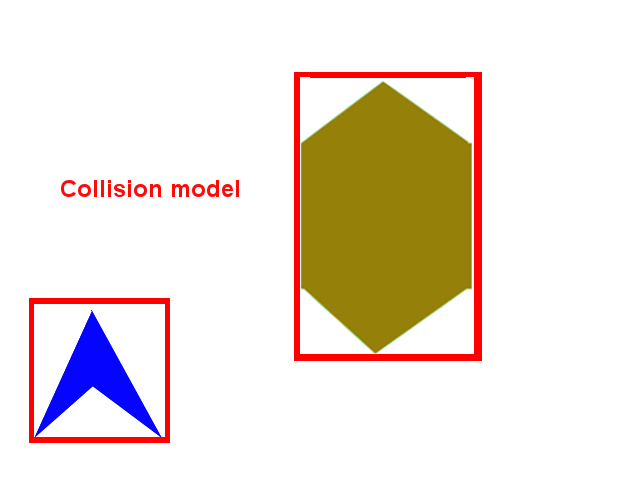
\includegraphics[width=0.5\textwidth]{Collision.png}
	\caption{Visualization of the Collision model.}
	\label{img:collision}
\end{figure}
\subsubsection{4. Slow the Player}
In the original ASTEROIDS game from 1979 the player is slowed down with time when moving. We decided to adopt this, so the game becomes more intuitive.
\end{document}
